\documentclass[tikz]{standalone}

\usetikzlibrary{positioning}

\begin{document}
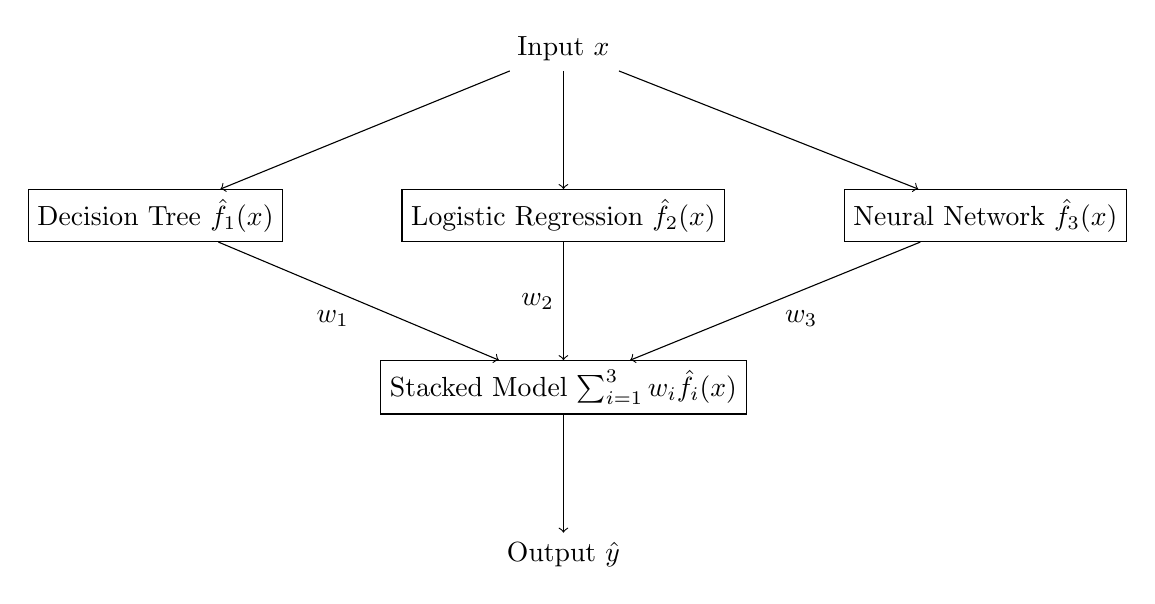
\begin{tikzpicture}[node distance=1.5cm]
    % Input layer
    \node (input) {Input $x$};

    % First layer
    \node[draw, rectangle, below=of input] (model2) {Logistic Regression $\hat{f}_2(x)$};
    \node[draw, rectangle, left=of model2] (model1) {Decision Tree $\hat{f}_1(x)$};
    \node[draw, rectangle, right=of model2] (model3) {Neural Network $\hat{f}_3(x)$};

    % Labels

    % Second layer
    \node[draw, rectangle, below=of model2] (stacked) {Stacked Model $\sum_{i=1}^3 w_i\hat{f}_i(x)$};

    % Output layer
    \node[below=of stacked] (output) {Output $\hat{y}$};

    % Arrows
    \draw[->] (input) -- (model1);
    \draw[->] (input) -- (model2);
    \draw[->] (input) -- (model3);
    \draw[->] (model1) -- (stacked) node[midway, below left] {$w_1$};
    \draw[->] (model2) -- (stacked) node[midway, left] {$w_2$};
    \draw[->] (model3) -- (stacked) node[midway, below right] {$w_3$};
    \draw[->] (stacked) -- (output);
\end{tikzpicture}
\end{document}
